\section{TINJAUAN PUSTAKA}

% Ubah konten-konten berikut sesuai dengan isi dari tinjauan pustaka

\subsection{Roket Luar Angkasa}

% Contoh input gambar dengan format *.jpg
\begin{figure} [ht] \centering
  % Nama dari file gambar yang diinputkan
  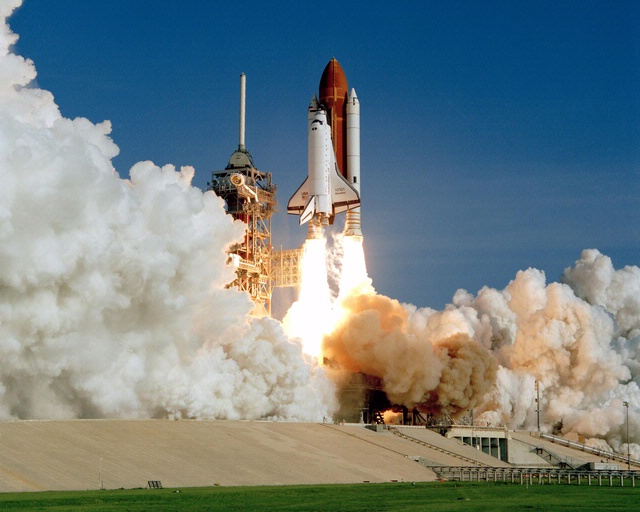
\includegraphics[scale=0.45]{gambar/space-shuttle.jpg}
  % Keterangan gambar yang diinputkan
  \caption{Peluncuran Pesawat Luar Angkasa \emph{Discovery}}
  % Label referensi dari gambar yang diinputkan
  \label{fig:spaceShuttle}
\end{figure}

% Contoh penggunaan referensi dari gambar yang diinputkan
Roket luar angkasa, seperti \emph{Discovery} \ref{fig:spaceShuttle}, merupakan \lipsum[2]

\subsection{Hukum Newton}

% Contoh penggunaan referensi dari pustaka
Newton pernah merumuskan \citep{newtonLaw} bahwa \lipsum[2]
% Contoh penggunaan referensi dari persamaan
Kemudian menjadi persamaan seperti pada persamaan \ref{eq:hukumPertama}.

% Contoh pembuatan persamaan
\begin{equation}
  % Label referensi dari persamaan yang dibuat
  \label{eq:hukumPertama}
  % Baris kode persamaan yang dibuat
  \sum \mathbf{F} = 0\; \Leftrightarrow\; \frac{\mathrm{d} \mathbf{v} }{\mathrm{d}t} = 0.
\end{equation}